\documentclass{beamer}

\usepackage[utf8]{inputenc}
\usepackage[T1]{fontenc}
\usepackage{graphicx}
\usepackage{listings}
\usepackage{xcolor}

\useinnertheme{uconn}
\useoutertheme[watermark=corner,logo=stacked]{uconn}
%\useoutertheme[footline=authorinstitute,subsection=true]{miniframes}
%\useoutertheme{sidebar}
\usecolortheme{default}
\usefonttheme{default}

\title[The introduction of Tensorflow]{The introduction of TensorFlow\\ with Applications in Sports Analytics}
\subtitle{Parallel session of UCSAS 2021}
\author[Jin]{Jun Jin, PhD candidate}
\institute[UConn]{Department of Statistics\\ University of Connecticut}
\date{\today}

\setlength{\parskip}{.5em}

\lstdefinestyle{Python}{
    language        = Python,
    basicstyle      = \tiny,
    keywordstyle    = \color{blue},
    keywordstyle    = [2] \color{teal}, % just to check that it works
    stringstyle     = \color{green},
    commentstyle    = \color{red}\ttfamily
}


\begin{document}

\lstset{
    frame       = single,
    numbers     = left,
    showspaces  = false,
    showstringspaces    = false,
}

\begin{frame}
\titlepage
\end{frame}


\begin{frame}{Table of contents}
\tableofcontents
\end{frame}

\section{Tensorflow}

\begin{frame}[fragile]{Advantage}
\uncover<1->
{
	\begin{picture}(0,0)(0,0)
		\put(10,-15)
		{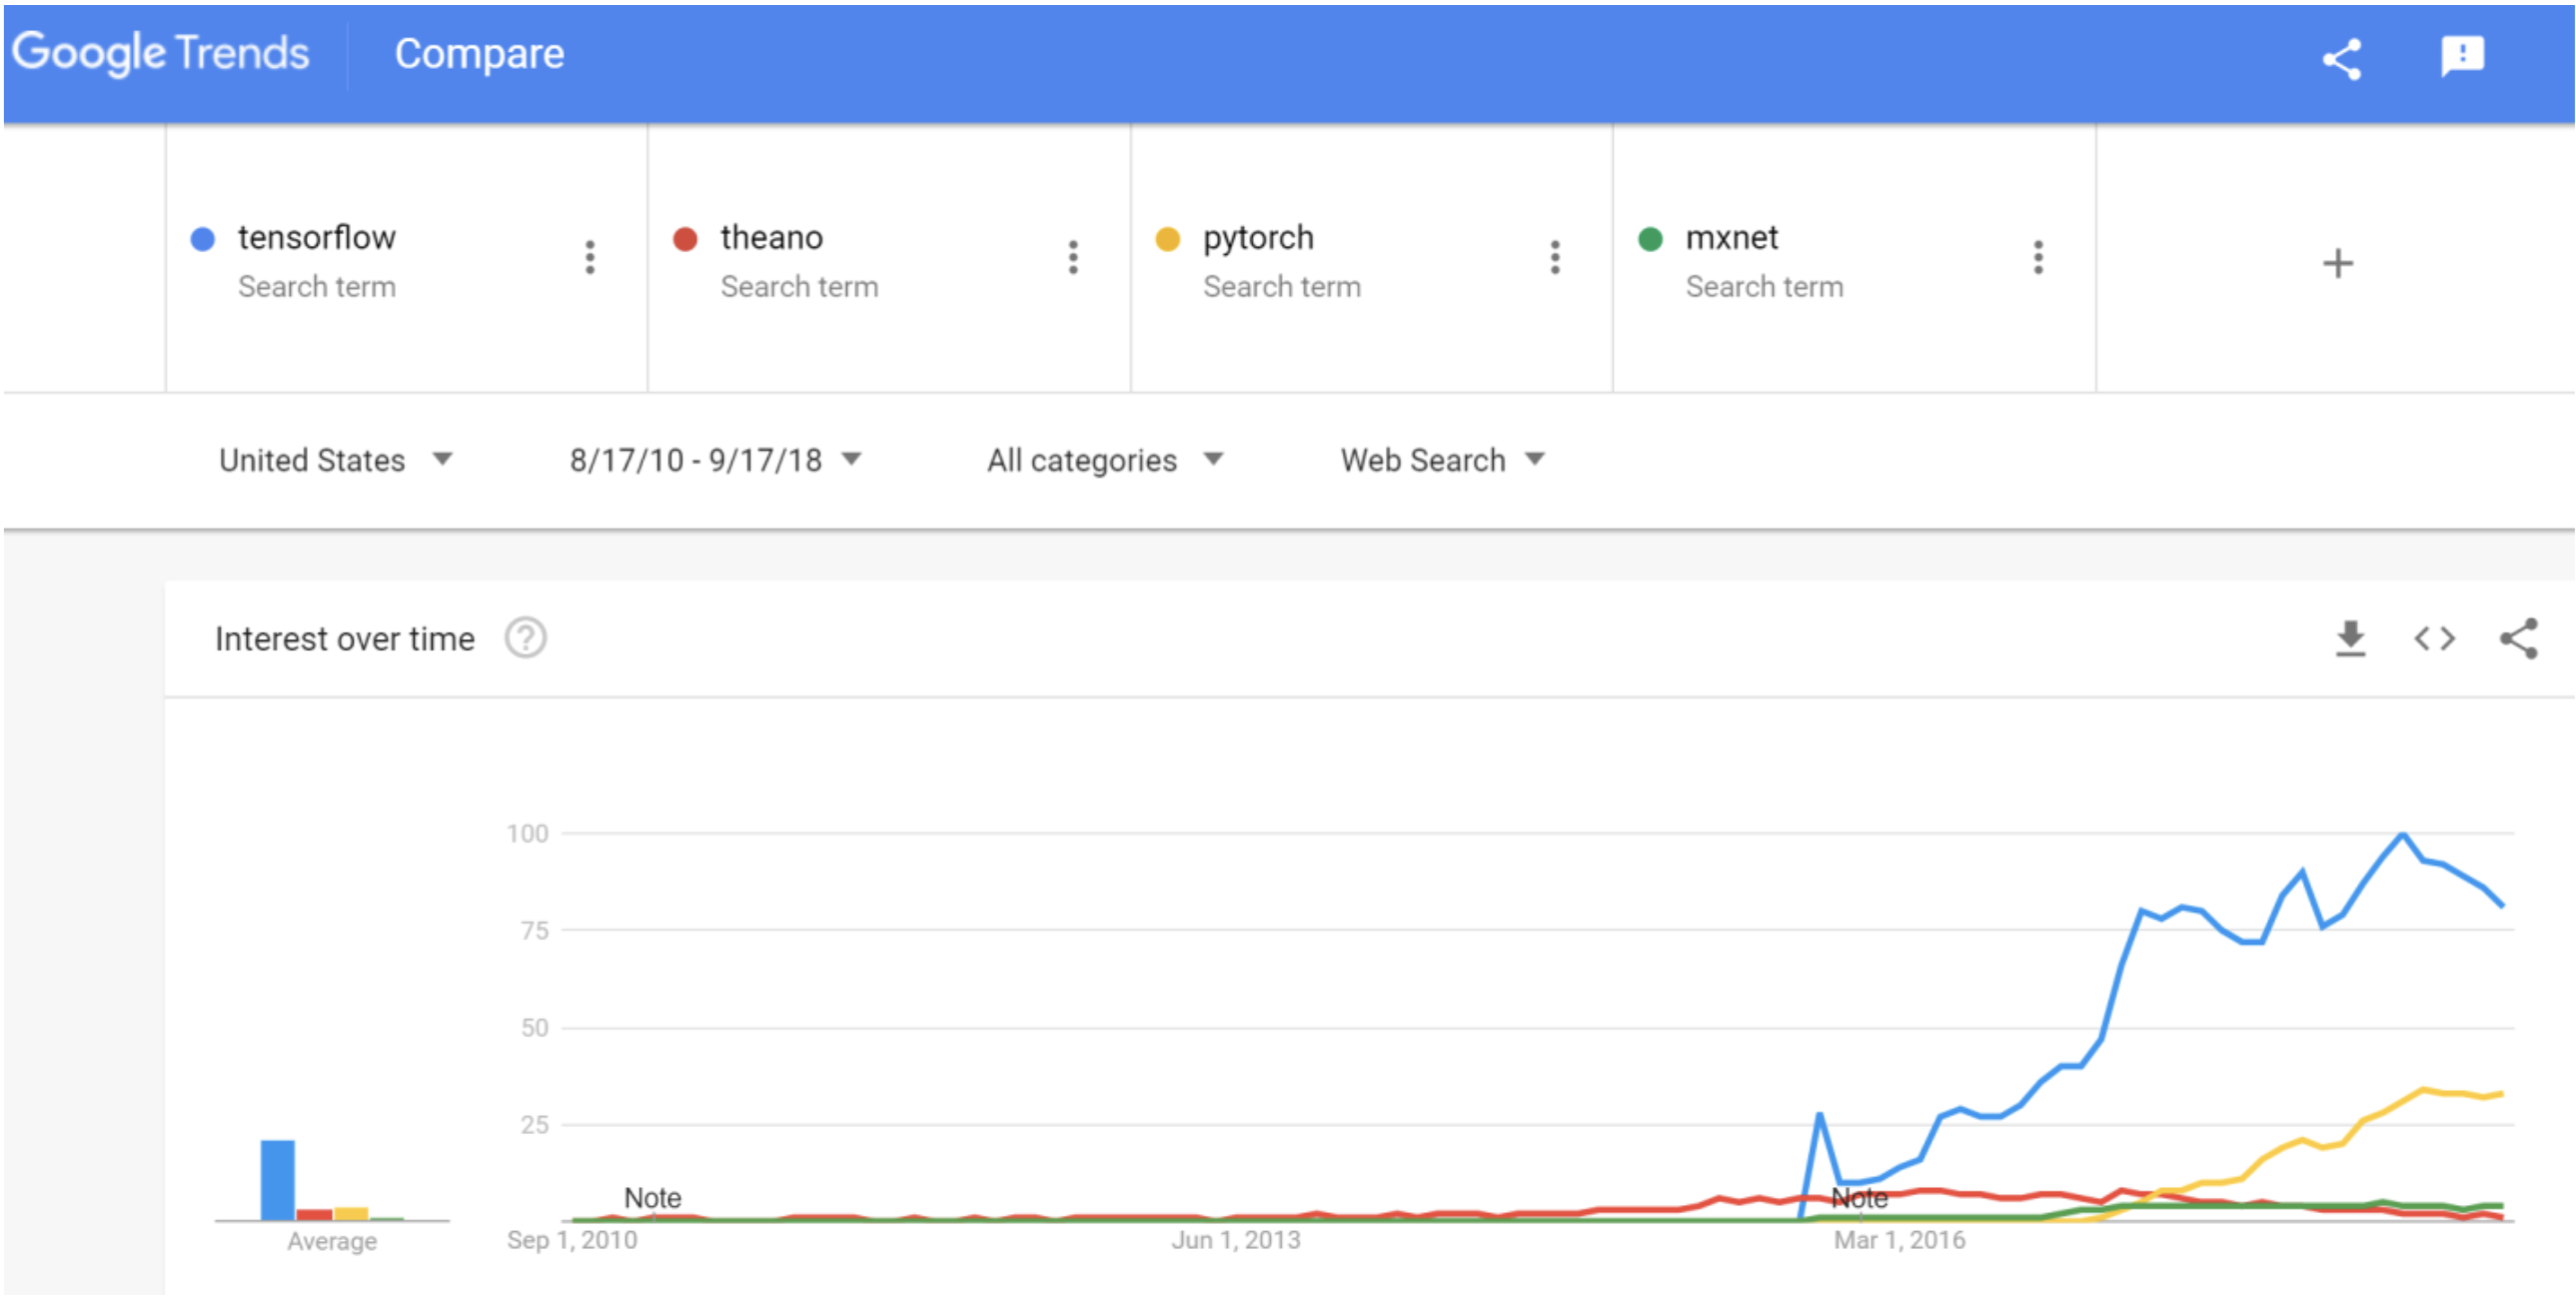
\includegraphics[width=7cm]{images/fig1.png}}
	\end{picture}
}

\uncover<2->
{
	\begin{picture}(0,0)(0,0)
		\put(90,-120)
		{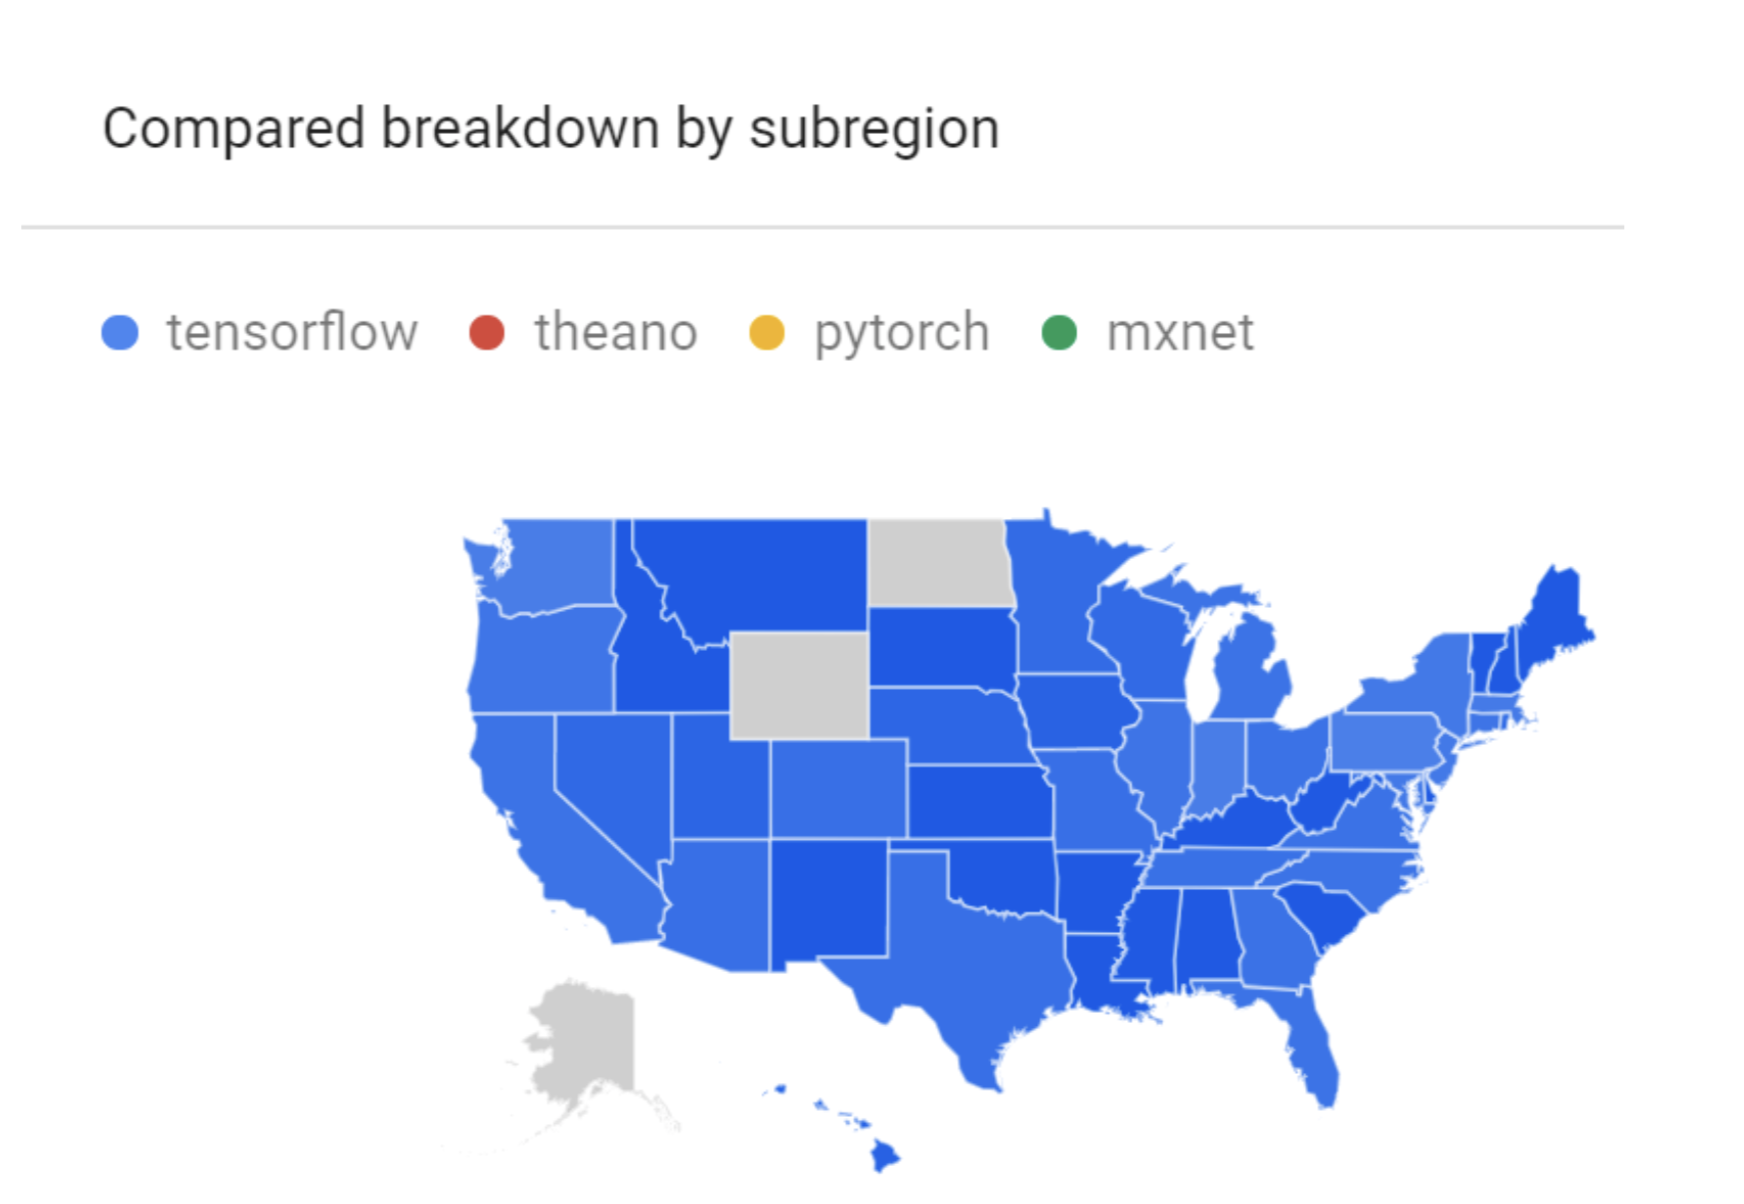
\includegraphics[width=7cm]{images/fig2.png}}
	\end{picture}
}

\end{frame}

\begin{frame}[fragile]{What is Tensor?}
\begin{itemize}
	\item Tensor is the data with dimension.
	\item 0-d tensor: scalar
	\begin{equation*}
	c = 5
	\end{equation*} 
	\item 1-d tensor: vector
	\begin{equation*}
	{\rm{c}} = \left( {\begin{array}{*{20}{c}}
1\\
 \vdots \\
5
\end{array}} \right)
	\end{equation*} 
	\item 2-d tensor: matrix
	\begin{equation*}
	{\rm{c}} = \left( {\begin{array}{*{20}{c}}
1& \cdots &5\\
 \vdots & \ddots & \vdots \\
5& \cdots &5
\end{array}} \right)
	\end{equation*}
\end{itemize}
\end{frame}


\begin{frame}[fragile]{Why Tensor special?}
\begin{itemize}
	\item Vector, matrix operations and gradient (derivative) are dominant in machine learning and deep learning.
	\begin{example}
	\begin{equation*}
	\left( {GD} \right):{\hat \beta ^{\left( {t + 1} \right)}} = {\hat \beta ^{\left( t \right)}} - \gamma \nabla {E_n}\left[ {\ell \left( {y,\hat y\left( {{{\hat \beta }^{\left( t \right)}}} \right)} \right)} \right]
	\end{equation*}
	\end{example}
	\item GPU structure leads to a powerful ability to solve linear tensor operations.
\end{itemize}
\end{frame}

\section{Installation}

\begin{frame}[fragile]{How to install Tensorflow in Python}
\begin{itemize}
	\item Anaconda management (GUI): click "environment" --> choose "Not installed" --> search "tensorflow"
	\item Anaconda Prompt: 
	\begin{verbatim}
    conda install tensorflow
	\end{verbatim}
	\item Pip:
	\begin{verbatim}
    pip install tensorflow 
	\end{verbatim} 
	\item Verify whether your installation is successful: (open jupyter notebook or run at .py file)
	\begin{lstlisting}[style = Python]
import tensorflow as tf
import tensorflow.compat.v1 as tfv1
tf.__version__
\end{lstlisting}
\end{itemize}
\end{frame}

\section{Concepts and Basis}

\begin{frame}[fragile]{3 key concepts in tensorflow programming}
\begin{itemize}
	\item Operations: Data operations like "matmul" (matrix multiplication), "add".
	\item Graph: Build GRAPH which represents the data flow of the computation.
	\item Session: Run SESSION which executes the operations on the graph.
\end{itemize}
\uncover<2->
{
	\begin{picture}(0,0)(0,0)
		\put(90,-80)
		{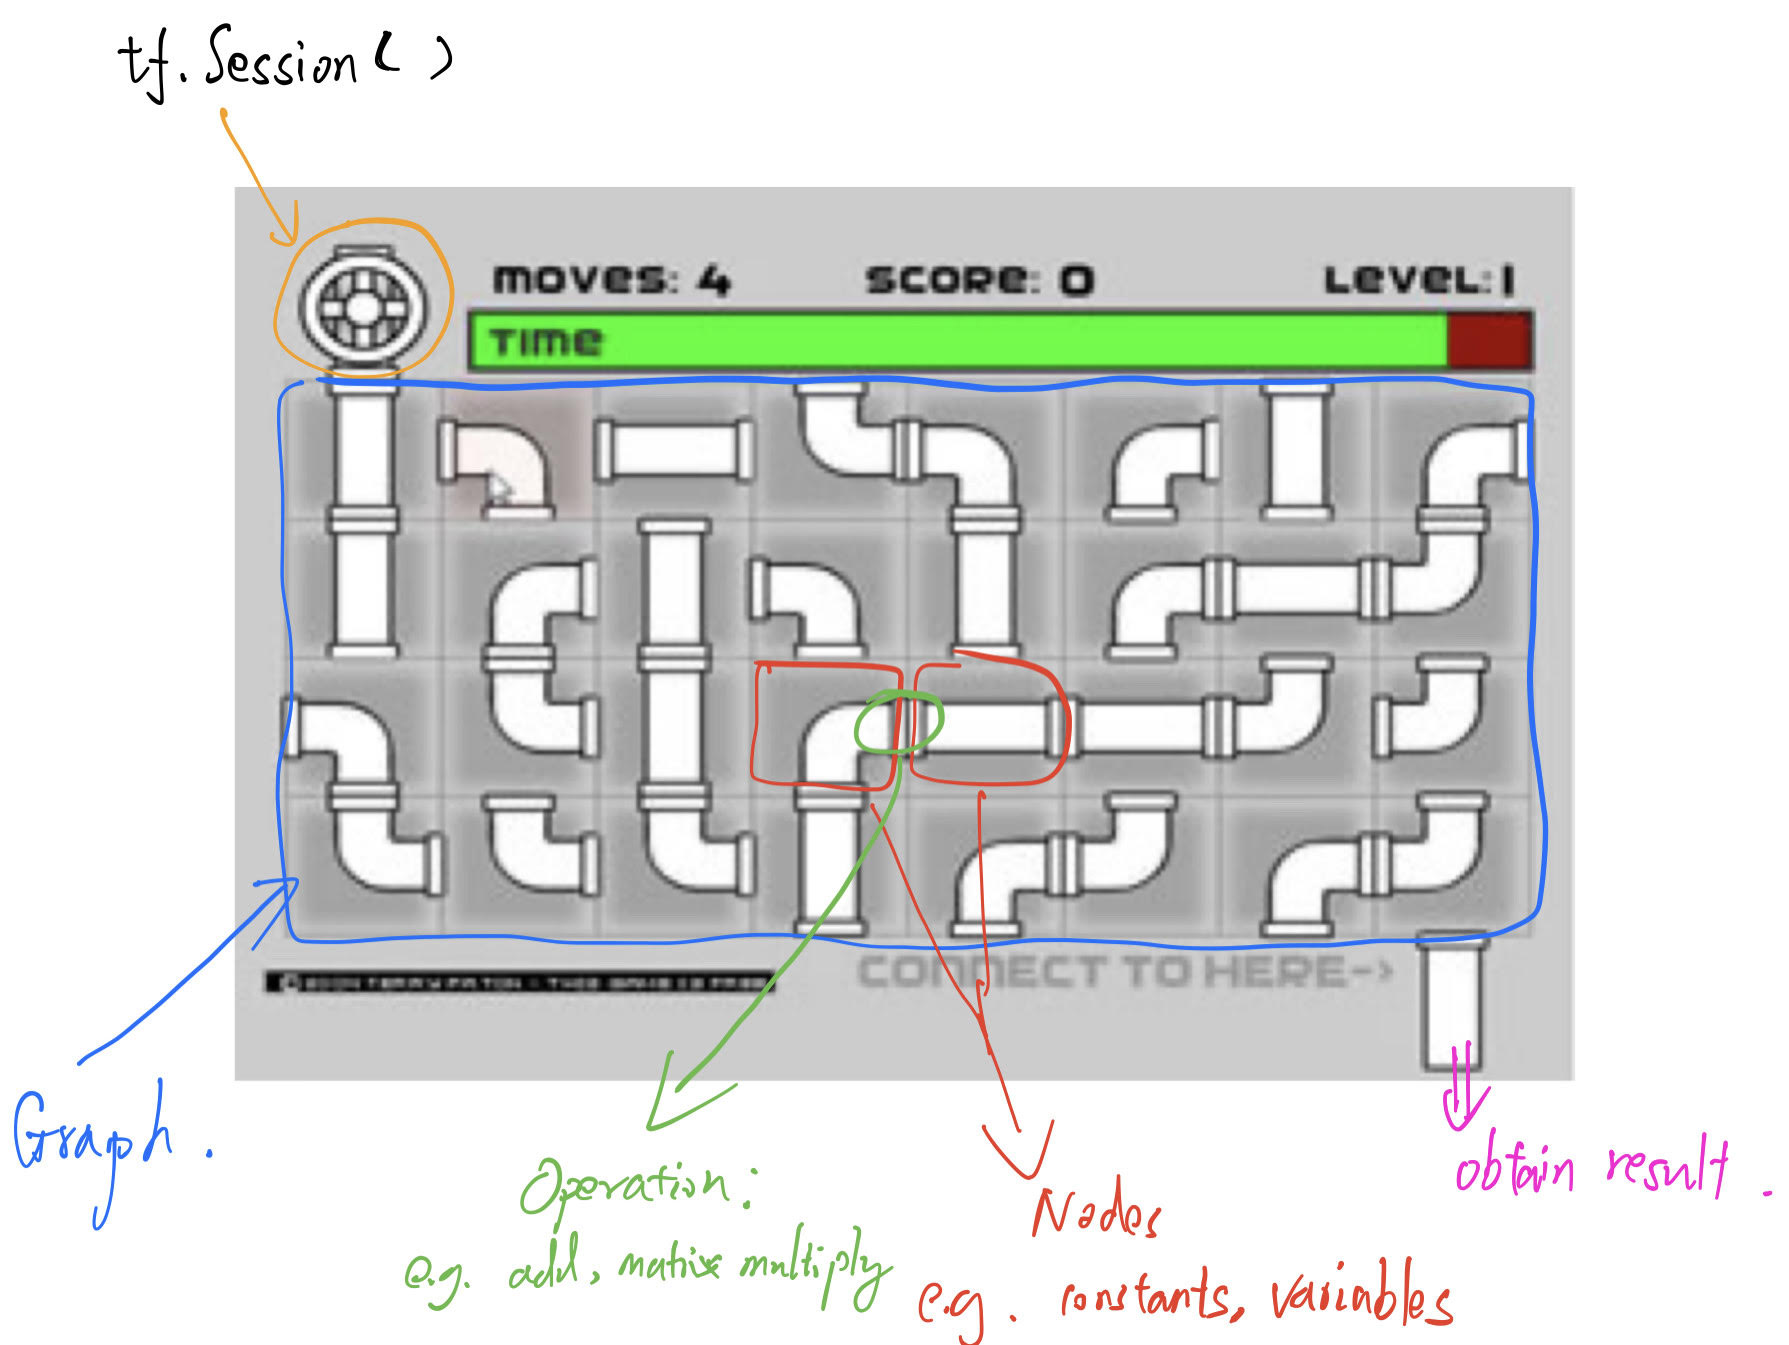
\includegraphics[width=9cm]{images/fig3.jpg}}
	\end{picture}
}
\end{frame}


\begin{frame}[fragile]{Tensorflow V1 versus V2}
\begin{itemize}
	\item V1: Nodes $ \to $  Operations $ \to$ Graph $\to$ Session $\to$ import the data
	\item V2: import the data $\to$ Nodes  $\to$ Operations (eager execution)
\end{itemize}
Pros and Cons:
\begin{itemize}
	\item V1 Pros: Integrity, a big picture of view
	\item V1 Cons: Lack of flexibility
	\item V2 Pros: Flexibility, you can always see the output step by step
	\item V2 Cons: Further efforts are frequently needed to pack the code up into a final package or class function
\end{itemize}
Therefore, V1 is frequently used in final delivery but V2 is good for debugging.
\end{frame}


\begin{frame}[fragile]{Tensorflow V1 versus V2}
Good news: V1 are V2 are both be accessible by tensorflow package.
\begin{itemize}
	\item Default is V2 (import tensorflow as tf)
	\item Use "import tensorflow.compat.v1 as tfv1" to call the functions and methods under V1
\end{itemize}
\end{frame}


\begin{frame}[fragile]{Basic widget: Constant}
The constant can be either scalar, vector, or matrix. It is just a concept which is opposite with variable. Variable can be changed in the future by using tf.assign() method, while the constant can not.
\begin{lstlisting}[style = Python]
s = tf.constant(2)
m = tf.constant([[1,2],[3,4]])
m = tf.constant([1,2,3,4],shape=[2,2])
\end{lstlisting}
With these two node, we can conduct a GRAPH and SESSION example. Here we use "tensorboard" for GRAPH and tf.Session() function for SESSION.
\end{frame}

\begin{frame}[fragile]{A simplest graph and session}
\begin{lstlisting}[style = Python]
g = tf.Graph()
with g.as_default():
    s = tf.constant(2)
    m = tf.constant([[1,2],[3,4]])
    mmul = s*m
g
\end{lstlisting}
Here, we have already completed a graph, to "open the faucet", we use tf.Session(), like:
\begin{lstlisting}[style = Python]
with tfv1.Session(graph=g) as sess:
    print(sess.run(mmul))
\end{lstlisting}
Finally, we get the result. Remark: The tf.Session() only exist in tensorflow v1, so we call this function under v1 platform.
\end{frame}

\begin{frame}[fragile]{Basic widget: Variable}
Variables are used to hold and update parameters. Another important difference with the constant is that it be treated as variable in the calculation of gradient. To create a variable, 
\begin{lstlisting}[style = Python]
w = tf.Variable(tf.ones((2,2))) # 2*2 matrix with all elements as 1
\end{lstlisting}
\begin{alertblock}{Alert}
The variable must be initialized immediately after "the data faucet is open" (i.e. tfv1.Session()).
\end{alertblock}
\begin{lstlisting}[style = Python]
with tfv1.Session() as sess:
    sess.run(tfv1.global_variables_initializer())
    print(sess.run(w))
\end{lstlisting}
\end{frame}

\begin{frame}[fragile]{Basic widget: Variable}
As we mentioned earlier, variable can be assigned with a new value. 
\begin{lstlisting}[style = Python]
with tfv1.Session() as sess:
    sess.run(tfv1.global_variables_initializer())
    print(sess.run(w))
    # Change w to a 2*2 matrix with all elements as 0
    sess.run(w.assign(tf.zeros((2,2)))) 
    print(sess.run(w))
\end{lstlisting}
\end{frame}


\begin{frame}[fragile]{Basic widget: Placeholder}
We can notice that although variable is more flexible than constant, it still need a initial value. In practice, sometimes the value of a parameter is determined by the actual data. So we need the placeholder to tell the PC, there is a variable, but I don't tell you the value, I will give you the value when I open the data faucet.
\begin{lstlisting}[style = Python]
import numpy as np
node1 = tfv1.placeholder(tf.float32,shape = [1,2])
node2 = tfv1.placeholder(tf.float32,shape = [1,2])
w_linear = tf.matmul(node1,w) + node2
with tfv1.Session() as sess:
    sess.run(tfv1.global_variables_initializer())
    print(sess.run(w))
    print(sess.run(w_linear,feed_dict={node1:np.matrix([1.0,2.0]),
    	node2:np.matrix([1.0,2.0])}))
\end{lstlisting}
\end{frame}

\begin{frame}[fragile]{Basic Operations}
Given $x$ and $y$,
\begin{itemize}
	\item x+y (element-wise): tf.add(x,y)
	\item x-y (element-wise): tf.subtract(x,y)
	\item x*y (element-wise): tf.multiply(x,y)
	\item x/y (element-wise): tf.divide(x,y)
	\item x*y (matrix style): tf.matmul(x,y)
	\item x<y (judgment): tf.less(x,y)
	\item x>y (judgment): tf.greater(x,y)
	\item x<=y (judgment): tf.less\_equal(x,y)
\end{itemize}
\end{frame}

\begin{frame}[fragile]{Gradient}
One of the most powerful thing for the Tensorflow is that it can calculate the gradient with a high flexibility and high speed. The core lines are:
\begin{lstlisting}[style = Python]
with tf.GradientTape() as tape:
	y1 = <Expression of x1, x2,...>
	y2 = <Expression of y1>
tape.gradient(y2,[x1,x2,...])
\end{lstlisting}
It returns the gradients of y2 with respect to x1, x2,... separately.
\begin{alertblock}{Alert}
The gradient operation can only return value when it is with respect to a trainable variable.
\end{alertblock}
\end{frame}


\begin{frame}[fragile]{Gradient}
\begin{lstlisting}[style = Python]
x = tf.Variable(3.0)
with tf.GradientTape() as tape:
  y = x**2
dy_dx = tape.gradient(y, x)
# dy = 2x * dx
with tfv1.Session() as sess:
    sess.run(tfv1.global_variables_initializer())
    print(sess.run(dy_dx))
\end{lstlisting}
\end{frame}


\begin{frame}[fragile]{Basic Logic: If}
The core line is:
\begin{lstlisting}[style = Python]
tf.cond(tf_statement,A,B)
\end{lstlisting}
It implement a function that if tf\_statement is true, then run A, otherwise, run B. By the way, it we want to choose from options more than 2, we can use tf.switch\_case() function, that is not included in this session.
\begin{example}
\begin{lstlisting}[style = Python]
t1 = tf.constant(1)
t2 = tf.constant(2)
def f1(): return t1+t2
def f2(): return t1-t2
res = tf.cond(t1<t2,f1,f2)
with tfv1.Session() as sess:
	print(sess.run(res))
\end{lstlisting}
It will return 1+2 as 1 is indeed less than 2.
\end{example}
\end{frame}

\begin{frame}[fragile]{Basic Logic: While}
The core line is:
\begin{lstlisting}[style = Python]
tf.while_loop(tf_statement,body,variables)
\end{lstlisting}
It implement a function that if tf\_statement is true, then run body, until tf\_statement is false. The variables position need a tuple or list including all the tensorflow variables needed in the body part and tf\_statement part. The loop will return the variables after the final iteration.
\begin{example}
\begin{lstlisting}[style = Python]
t1 = tf.constant(1)
t2 = tf.constant(5)
body = (tf.add(t1,1),t2)
def cond(t1,t2): return t1<t2
def body(t1,t2): 
    t1 = tf.add(t1,1)
    return (t1,t2)
res = tf.while_loop(cond,body,(t1,t2))
with tfv1.Session() as sess:
    print(sess.run(res))
\end{lstlisting}
\end{example}
\end{frame}


\section{Framework}

\begin{frame}[fragile]{Framework}
With all the knowledge we have learned, we now turn to something practical. Generally, we'd like the model training and model predicting to be simple, we prefer a calling style likes the following:
\begin{lstlisting}[style = Python]
model = model_creation_function()
\end{lstlisting}
Firstly, we use a certain model\_creation\_function to implement the initialization of variables and parameters we need, actually, it create a \emph{class} data in Python. Then:
\begin{lstlisting}[style = Python]
model.fit(x=...,y=...)
\end{lstlisting}
we hope this class type model hold a function called "fit", and the input should be $x$ and $y$ (in most cases of supervised learning). Finally,
\begin{lstlisting}[style = Python]
predict_value = model.predict(x=...)
\end{lstlisting}
we also hope this class type model hold functions for prediction, evaluation and etc.
\end{frame}

\section{Example with simulated data (Regression)}

\begin{frame}[fragile]{Linear Regression Excersice}
Given ${\rm{X}} \in {{\rm{R}}^{n * 2}}$ and $Y \in {R^n}$, find a $\beta  \in {R^2}$ which is the OLS estimator for model 
\begin{equation*}
Y = X\beta  + \varepsilon ,\varepsilon  \sim N\left( {0,{\sigma ^2}} \right).
\end{equation*}
Key idea:
\par
Implement the (loss) objective function:
\begin{equation*}
L\left( \beta  \right) = {\left\| {Y - X\beta } \right\|^2}.
\end{equation*}
Give any initial value ${{\hat \beta }^{\left( 0 \right)}} = {\left( {0,0} \right)^T}$ and use the Gradient Descent method. The solution of this exercise is attached in the code directory. 
\end{frame}

\section{Example with real-world data (Classification)}

\begin{frame}[fragile]{Sport data analysis}
In this section, our goal is to make prediction on the result of football matches based on the twitter sentiment of 200 games from the English Premier League. Data is from the \href{https://betsentiment.com/}{\tt \textcolor{blue}{Betsentiment.com}} with structure (key columns):
\begin{itemize} 
	\item home: The home team
	\item away: The away team
	\item sentiment\_score\_st\_a: The sentiment score of home team at the starting time of bet
	\item sentiment\_score\_st\_b: The sentiment score of away team at the starting time of bet
	\item sentiment\_score\_lt\_a: The sentiment score of home team at the last time of bet
	\item sentiment\_score\_lt\_b: The sentiment score of away team at the last time of bet
\end{itemize}
\end{frame}


\begin{frame}[fragile]{Sport data analysis}
\begin{itemize}
	\item wgted\_players\_sentiment\_a: The weighted players sentiment score of home team
	\item wgted\_players\_sentiment\_b: The weighted players sentiment score of away team
	\item wgted\_players\_sentiment\_st\_a: The weighted players sentiment score of home team at the starting time of bet
	\item wgted\_players\_sentiment\_st\_b: The weighted players sentiment score of away team at the starting time of bet
	\item final\_result: The final result (home win: 1; home loss: 2, tie: 3)
\end{itemize}
We run several neural network models with different structures, whose code is attached in the code directory. Thank you for listening. \oakleaf
\end{frame}



\section{Thanks}


\begin{frame}{Useful info}

The material of this session is in \href{https://github.com/brucejunjin/ucsas2020}{\tt \textcolor{blue}{Session Material}}.
\par
Our department website is \href{https://stat.uconn.edu/}{\tt \textcolor{blue}{Department of Statistics}}.
\par
Our website for statistical data science lab at Uconn is \href{https://statds.org/}{\tt \textcolor{blue}{Data Science Lab}}.

\end{frame}


\end{document}

